\documentclass[a4paper,12pt]{article}
\usepackage{float}
\usepackage[table]{xcolor} % Para colorir as linhas da tabela
\usepackage{array} % Para melhorar a formatação de tabelas
\usepackage[brazil]{babel}
\usepackage[utf8]{inputenc}
\usepackage{indentfirst}
\usepackage{amsmath}
\usepackage{graphicx}
\usepackage{animate}
\usepackage[font=footnotesize, labelfont=bf, listformat=empty]{caption}
\usepackage{geometry}
\usepackage{listings}
\usepackage{lastpage}
\usepackage{subcaption}
\usepackage[skins,xparse,breakable]{tcolorbox}
\usepackage{longtable}
\usepackage{minted}
\usepackage{titlesec}
\usepackage{fancyhdr}
\usepackage{setspace}
\usepackage[colorlinks=true, allcolors=black]{hyperref}

% Configurações de margens e espaçamento
\geometry{a4paper, left=3cm, right=2cm, top=3cm, bottom=2cm}
\setlength{\parindent}{1.25cm}
\onehalfspacing

% Configurações de títulos
\titleformat{\section}{\normalfont\large\bfseries}{\thesection}{1em}{}
\titleformat{\subsection}{\normalfont\bfseries}{\thesubsection}{1em}{}
\titleformat{\subsubsection}{\normalfont\itshape}{\thesubsubsection}{1em}{}

% Configurações de listagens
\renewcommand{\listingscaption}{Código}
\newenvironment{code}{\captionsetup{type=listing}}{}

% Configurações de cores
\definecolor{LightSeaGreen}{rgb}{0.1255, 0.6980, 0.6667}
\definecolor{whitesmoke}{rgb}{0.96, 0.96, 0.96}
\definecolor{cinza}{RGB}{160, 160, 160}
\definecolor{cinza_claro}{RGB}{240, 240, 240} % Cinza claro

% Configurações do minted para VHDL
\setminted[VHDL]{
    style=vs,
    linenos=true,
    breaklines=true,
    mathescape=true,
    bgcolor=cinza_claro,
    breakanywhere=true,
}

\newcommand{\hex}[1]{\textcolor{green!50!black}{#1}}

% Configurações de cabeçalho e rodapé
\pagestyle{fancy}
\fancyhf{}
\fancyhead[L]{\footnotesize{Laboratório de Sistemas Digitais - ENE0040}}
\fancyhead[R]{\footnotesize{2025/1 - Turma 07}}
\fancyfoot[R]{\footnotesize{Página \ \thepage \ de \pageref{LastPage}}}
\fancyfoot[L]{\footnotesize{Relatório do Experimento 3}}

% Adiciona uma linha preta acima do rodapé
\renewcommand{\footrulewidth}{0.4pt} % Espessura da linha
\renewcommand{\footrule}{\vbox to 0pt{\hrule width \textwidth height \footrulewidth \vss}} % Desenha a linha

% Novo Comando para chamar a capa
\newcommand{\capa}{
    \begin{titlepage}
        \begin{center}
            {\large \textbf{ENE0040 - Laboratório de Sistemas Digitais - Turma 07}} \\
            \vspace{3cm}
            {\Huge \textbf{Relatório do Experimento 3}} \\[1em]
            {\large \textbf{Autor:} Henrique Morcelles Salum} \\[0.5em]
            {\large \textbf{Matrícula:} 232003008} \\
            \vfill
            {\Large \textbf{Universidade de Brasília - UnB}} \\[0.75em]
            {\large \textbf{Departamento de Engenharia Elétrica - ENE}} \\
        \end{center}
    \end{titlepage}
}

\begin{document}

\capa

% Sumário
\newpage
\tableofcontents
\newpage

% Introdução
\section{Introdução}

\subsection{Sobre o Experimento}
\paragraph{}
Este experimento é composto por duas tarefas, em ambas, deve-se implementar circuitos lógicos com VHDL e simulá-los por meio do software ModelSim, da Intel. As especificidades de cada tarefa serão exploradas a seguir.

\subsubsection{Multiplexador 8 para 1}
\paragraph{}
Na primeira tarefa, devemos escrever, utilizando atribuições condicionais \textit{when-else}, uma entidade com dois vetores de entrada $S$, de três bits, e $D$, de oito bits, e um sinal de saída $Y$ que descreva um Mux 8x1. A tabela-verdade do sistema é a que segue:

\begin{table}[H]
    \footnotesize
    \centering
    \begin{tabular}{|c|c|c|c|}
        \hline
        \rowcolor{black}
        \textcolor{white}{$S_2$} & \textcolor{white}{$S_1$} & \textcolor{white}{$S_0$} & \textcolor{white}{Saída} \\ \hline
        0 & 0 & 0 & $D_0$ \\ \hline
        \rowcolor{cinza}
        0 & 0 & 1 & $D_1$ \\ \hline
        0 & 1 & 0 & $D_2$ \\ \hline
        \rowcolor{cinza}
        0 & 1 & 1 & $D_3$ \\ \hline
        1 & 0 & 0 & $D_4$ \\ \hline
        \rowcolor{cinza}
        1 & 0 & 1 & $D_5$ \\ \hline
        1 & 1 & 0 & $D_6$ \\ \hline
        \rowcolor{cinza}
        1 & 1 & 1 & $D_7$ \\ \hline
    \end{tabular}
    \caption{Tabela-verdade do multiplexador 8x1}
    \vspace{-5pt}
\end{table}


\subsubsection{Decodificador 4 para 16}
\paragraph{}
Na segunda tarefa, a entidade que devemos implementar em VHDL, utilizando atribuições seletivas \textit{with-select}, é um decodificador 4 para 16. Ele tem um vetor de entrada $A$, de quatro bits, e um vetor de saída $Y$ de 16 bits. A tabela-verdade é a que segue:

\begin{table}[H]
    \centering
    \footnotesize
    \setlength{\tabcolsep}{3pt}
    \begin{tabular}{|cccc|cccccccccccccccc|c|}
        \hline
        \rowcolor{black}
        \multicolumn{4}{|c|}{\textbf{\textcolor{white}{Entrada}}} & \multicolumn{17}{|c|}{\textbf{\textcolor{white}{Saída}}} \\ \hline
        \rowcolor{black}
        \textcolor{white}{$A_3$} & \textcolor{white}{$A_2$} & \textcolor{white}{$A_1$} & \textcolor{white}{$A_0$} & \textcolor{white}{$Y_{15}$} & \textcolor{white}{$Y_{14}$} & \textcolor{white}{$Y_{13}$} & \textcolor{white}{$Y_{12}$} & \textcolor{white}{$Y_{11}$} & \textcolor{white}{$Y_{10}$} & \textcolor{white}{$Y_9$} & \textcolor{white}{$Y_8$} & \textcolor{white}{$Y_7$} & \textcolor{white}{$Y_6$} & \textcolor{white}{$Y_5$} & \textcolor{white}{$Y_4$} & \textcolor{white}{$Y_3$} & \textcolor{white}{$Y_2$} & \textcolor{white}{$Y_1$} & \textcolor{white}{$Y_0$} & \textbf{\textcolor{white}{Hex}} \\ \hline
        0 & 0 & 0 & 0 & 0 & 0 & 0 & 0 &  0 & 0 & 0 & 0 & 0 & 0 & 0 & 0 &  0 & 0 & 0 & 1 & $0001h$ \\ \hline
        \rowcolor{cinza}
        0 & 0 & 0 & 1 & 0 & 0 & 0 & 0 & 0 & 0 & 0 & 0 & 0 & 0 & 0 & 0 & 0 & 0 & 1 & 0 & $0002h$ \\ \hline
        0 & 0 & 1 & 0 & 0 & 0 & 0 & 0 & 0 & 0 & 0 & 0 & 0 & 0 & 0 & 0 & 0 & 1 & 0 & 0 & $0004h$ \\ \hline
        \rowcolor{cinza}
        0 & 0 & 1 & 1 & 0 & 0 & 0 & 0 & 0 & 0 & 0 & 0 & 0 & 0 & 0 & 0 & 1 & 0 & 0 & 0 & $0008h$ \\ \hline
        0 & 1 & 0 & 0 & 0 & 0 & 0 & 0 & 0 & 0 & 0 & 0 & 0 & 0 & 0 & 1 & 0 & 0 & 0 & 0 & $0010h$ \\ \hline
        \rowcolor{cinza}
        0 & 1 & 0 & 1 & 0 & 0 & 0 & 0 & 0 & 0 & 0 & 0 & 0 & 0 & 1 & 0 & 0 & 0 & 0 & 0 & $0020h$ \\ \hline
        0 & 1 & 1 & 0 & 0 & 0 & 0 & 0 & 0 & 0 & 0 & 0 & 0 & 1 & 0 & 0 & 0 & 0 & 0 & 0 & $0040h$ \\ \hline
        \rowcolor{cinza}
        0 & 1 & 1 & 1 & 0 & 0 & 0 & 0 & 0 & 0 & 0 & 0 & 1 & 0 & 0 & 0 & 0 & 0 & 0 & 0 & $0080h$ \\ \hline
        1 & 0 & 0 & 0 & 0 & 0 & 0 & 0 & 0 & 0 & 0 & 1 & 0 & 0 & 0 & 0 & 0 & 0 & 0 & 0 & $0100h$ \\ \hline
        \rowcolor{cinza}
        1 & 0 & 0 & 1 & 0 & 0 & 0 & 0 & 0 & 0 & 1 & 0 & 0 & 0 & 0 & 0 & 0 & 0 & 0 & 0 & $0200h$ \\ \hline
        1 & 0 & 1 & 0 & 0 & 0 & 0 & 0 & 0 & 1 & 0 & 0 & 0 & 0 & 0 & 0 & 0 & 0 & 0 & 0 & $0400h$ \\ \hline
        \rowcolor{cinza}
        1 & 0 & 1 & 1 & 0 & 0 & 0 & 0 & 1 & 0 & 0 & 0 & 0 & 0 & 0 & 0 & 0 & 0 & 0 & 0 & $0800h$ \\ \hline
        1 & 1 & 0 & 0 & 0 & 0 & 0 & 1 & 0 & 0 & 0 & 0 & 0 & 0 & 0 & 0 & 0 & 0 & 0 & 0 & $1000h$ \\ \hline
        \rowcolor{cinza}
        1 & 1 & 0 & 1 & 0 & 0 & 1 & 0 & 0 & 0 & 0 & 0 & 0 & 0 & 0 & 0 & 0 & 0 & 0 & 0 & $2000h$ \\ \hline
        1 & 1 & 1 & 0 & 0 & 1 & 0 & 0 & 0 & 0 & 0 & 0 & 0 & 0 & 0 & 0 & 0 & 0 & 0 & 0 & $4000h$ \\ \hline
        \rowcolor{cinza}
        1 & 1 & 1 & 1 & 1 & 0 & 0 & 0 & 0 & 0 & 0 & 0 & 0 & 0 & 0 & 0 & 0 & 0 & 0 & 0 & $8000h$ \\ \hline
    \end{tabular}
    \caption{Tabela-verdade do Decodificador 4 para 16}
    \label{tab:dec4x16}
    \vspace{-20pt}
\end{table}

\paragraph{}
Note que, na \autoref{tab:dec4x16}, há uma coluna para a representação em hexadecimal da saída. Quando lidamos com representações binárias muito grandes, é conveniente utilizar essa representação pois, se um número em sua representação binária tem $n$ casas, em sua representação hexadecimal ele terá $log_2 n$. Além disso, a conversão de binário para hexadecimal é muito fácil: cada algarismo da representação hexadecimal é substituído pela sua representação binária - que tem quatro bits, já que o algarismo hexadecimal de maior valor é o $F_{16}$, que tem valor $15_{10} = 1111_{2}$ - e pronto! Representações hexadecimais serão utilizadas nos códigos em VHDL nesse experimento.

\subsection{Introdução Teórica}

\subsubsection{Multiplexador 8 para 1}
\paragraph{}
Um multiplexador, também chamado de Mux, é um dispositivo digital que seleciona uma entre várias entradas de dados como saída. Essencialmente, o multiplexador atua como um ``comutador'' controlado por entradas de seleção, determinando qual sinal será encaminhado para a saída. Esse dispositivo é extensivamente usado no projeto de máquinas de estados, pois ele é muito conveniente quando é necessário implementar diferentes lógicas a depender do estado atual.

\paragraph{}
Para entender esse dispositivo, podemos separar as entradas entre entradas de dados, que são informações a serem selecionadas, e as entradas de seleção, que são utilizadas para escolher qual das entradas de dados será enviada para a saída. O número de entradas de seleção pode ser calculado em função do número de entradas de dados $n$ pela função:
\[
f(n) = \lceil \log_2n \rceil
\]

\paragraph{}
Nesse experimento, implementamos, especificamente, um multiplexador 8 para 1, ou seja, um multiplexador com oito entradas de dados e, consequentemente, $\log_2 8 = 3$ entradas de seleção, além de um sinal de saída.

\begin{figure}[H]
    \centering
    \includegraphics[width=0.25\textwidth]{Imagens/multiplexador.png}
    \caption{Representação externa do multiplexador 8 x 1}
    \label{fig:Mux_externa}
\end{figure}

\subsubsection{Decodificador 4 para 16}
\paragraph{}
O decodificador, chamado de Dec, é um circuito combinatório com $n$ bits de entrada e $2^n$ bits de saída que, para cada combinação dos bits de entrada, ativa apenas um bit de saída. Por convenção, o bit ativado costuma estar na posição representada pelos bits de entrada. Nesse experimento, implementamos, especificamente, o Dec 4x16.

\begin{figure}[H]
    \centering
    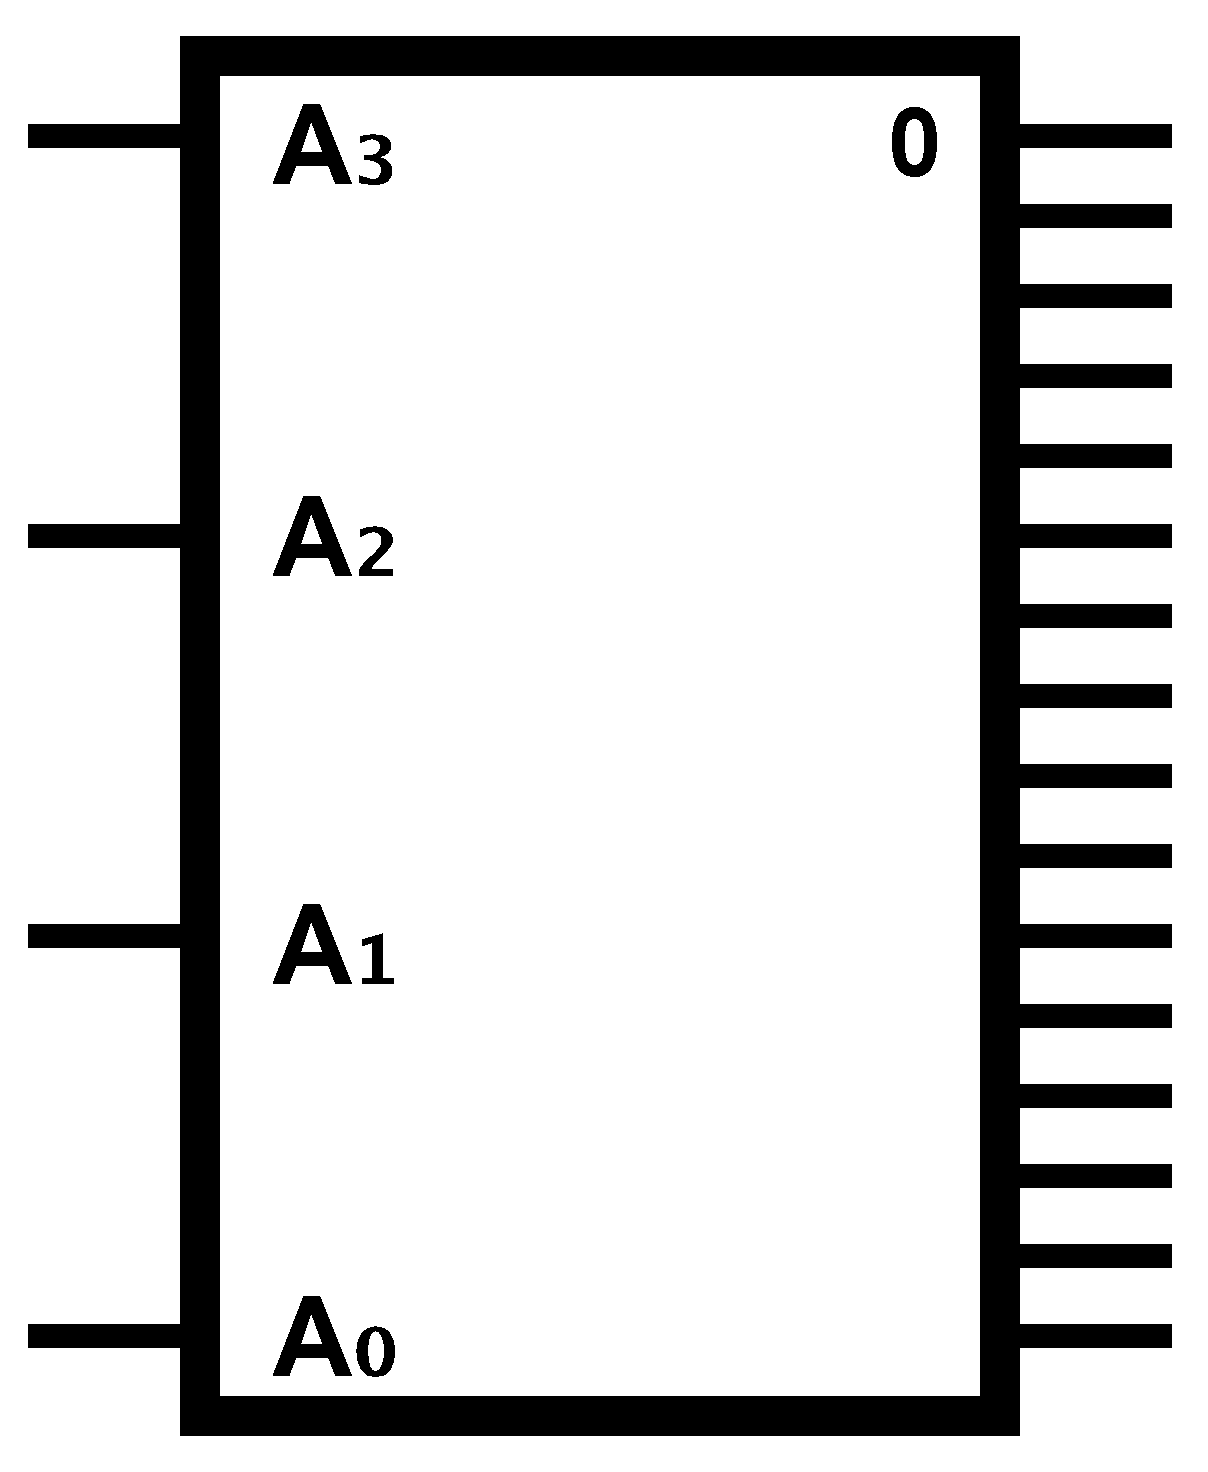
\includegraphics[width=0.25\linewidth]{Imagens/Decodificador.png}
    \caption{Representação externa do decodificador 4 x 16}
    \label{fig:dec4x16}
\end{figure}

\paragraph{}
Olhando para a \autoref{tab:dec4x16}, podemos perceber que cada saída do decodificador representa uma combinação dos $n$ bits de entrada, ou seja, um \textit{mintermo} dos bits de entrada. Esse fato justifica o interesse no decodificador: desde que toda função pode ser decomposta na soma dos mintermos que representam as linhas da tabela-verdade que essa função ativa, podemos fazer um $OR$ entre saídas específicas do Dec para gerar qualquer função booleana. Por exemplo:
\[
f(w, x, y, z) = \overline{w} \ \overline{x} \ \overline{y} \ \overline{z} + \overline{w} \ \overline{x} \ \overline{y} z + \overline{w} x \overline{y} \ \overline{z} + \overline{w}x \overline{y} z + \overline{w}xy\overline{z}
\]
\[
= \sum_{wxyz}m(0,1,4,5,6)
\]
Podemos implementar $f(w, x, y, z)$ da seguinte forma:

\begin{figure}[H]
    \centering
    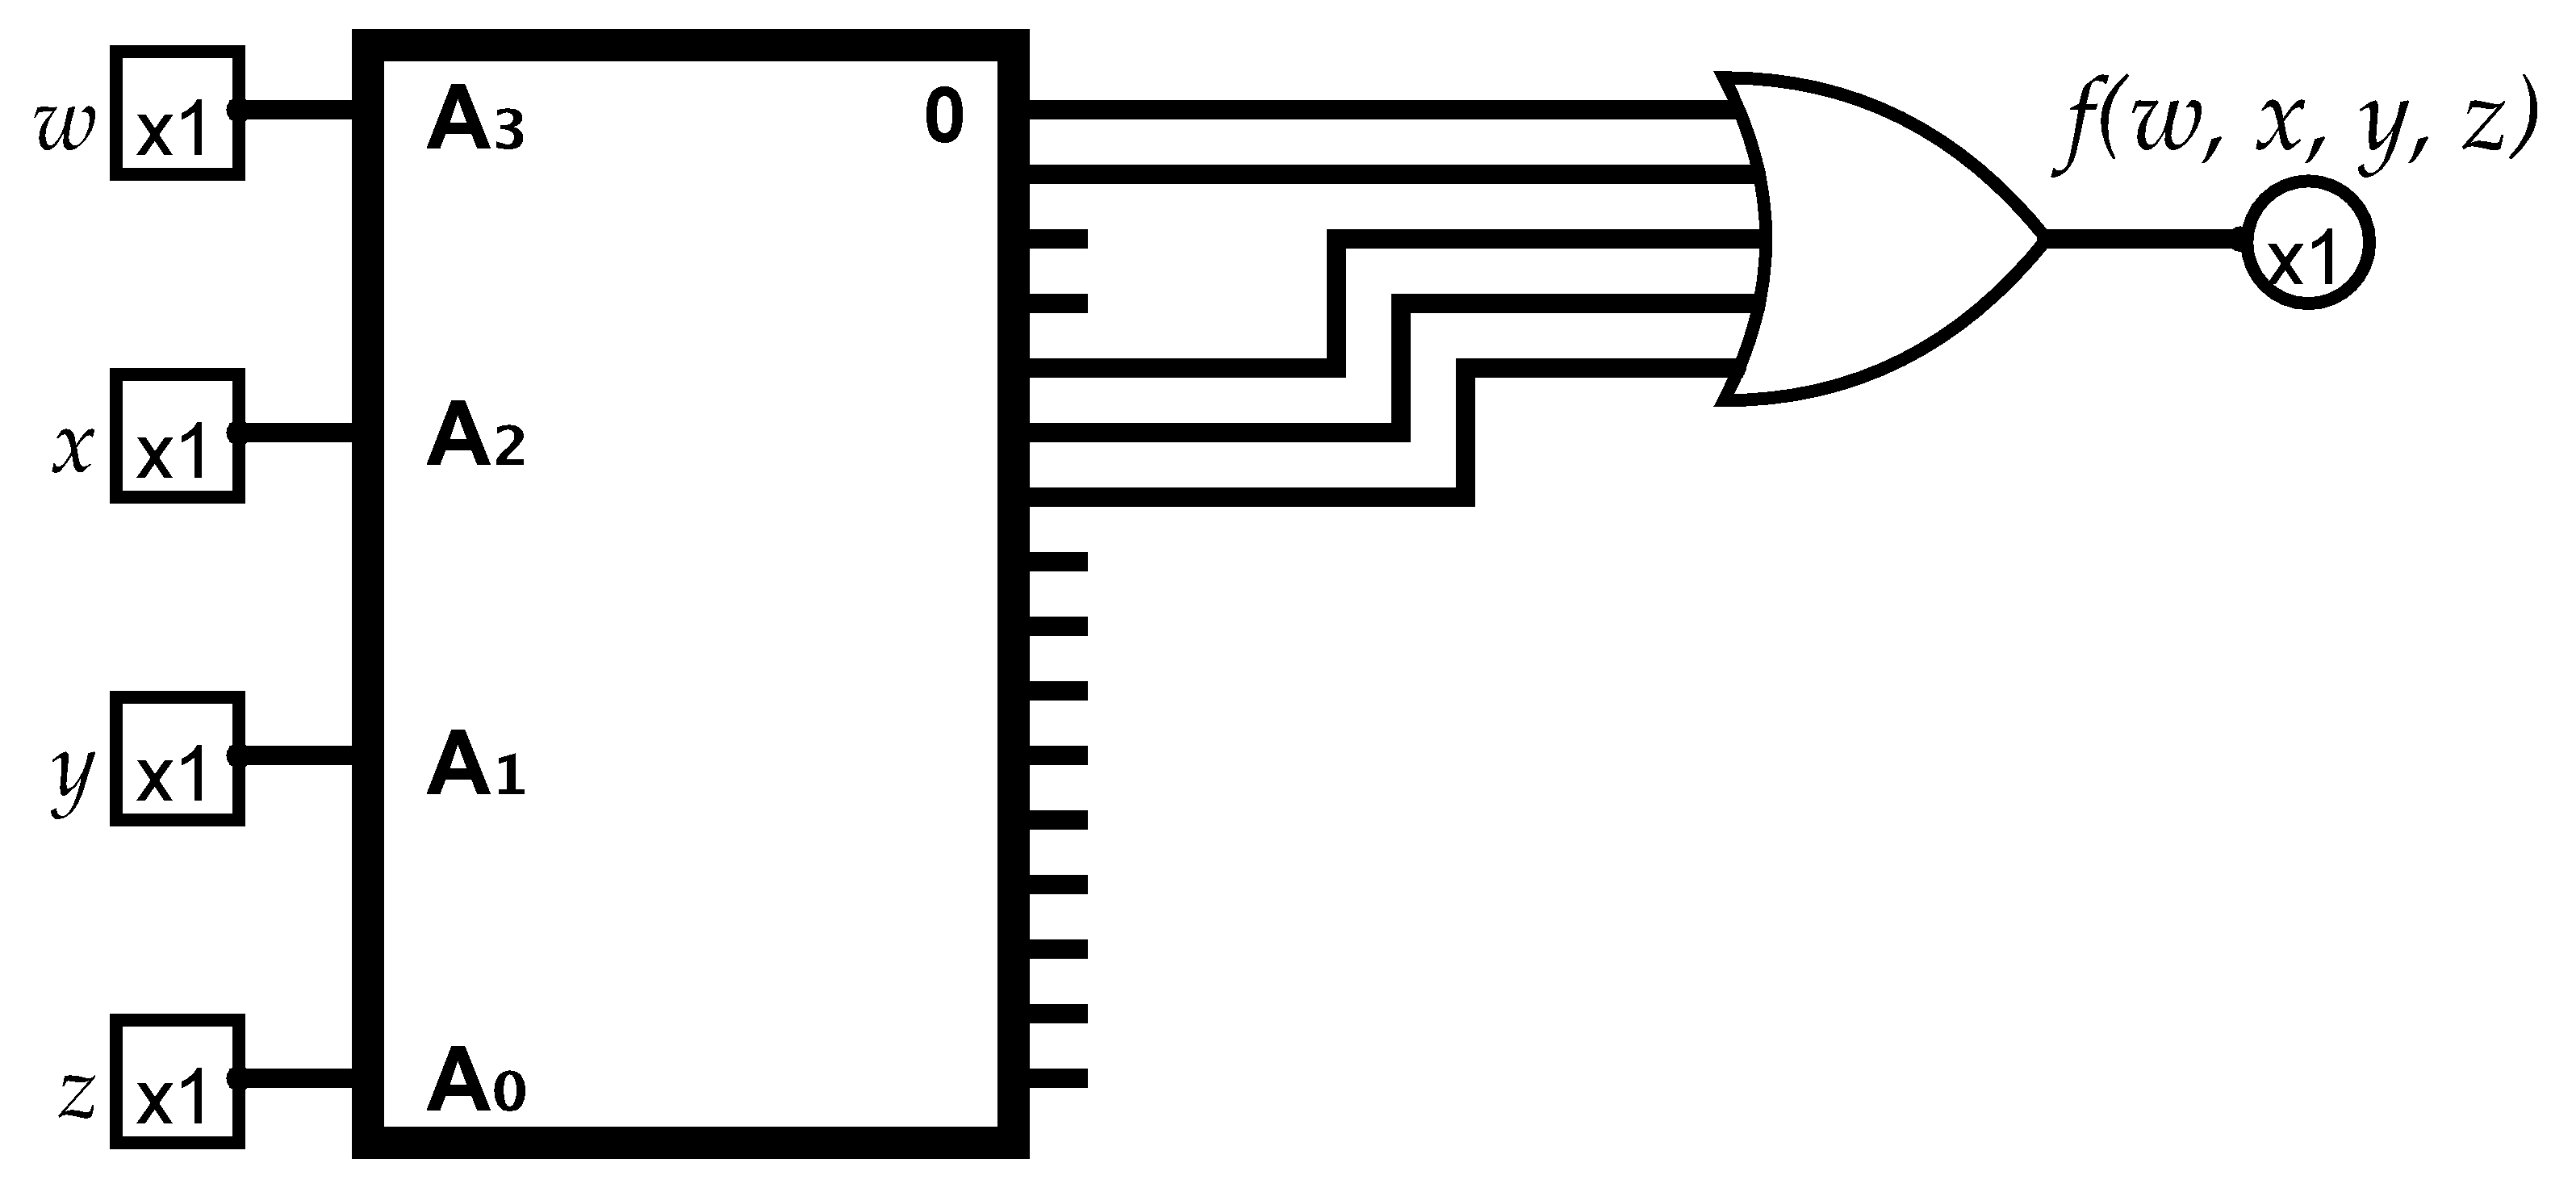
\includegraphics[width=0.9\linewidth]{Imagens/ExemploDec.png}
    \label{fig:enter-label}
\end{figure}


\section{Códigos}
\paragraph{}
Nessa seção, serão apresentados os códigos desenvolvidos, em VHDL, para implementar os sistemas digitais apresentados na introdução. Aqui, alguns comentários foram suprimidos para melhor apresentação, mas os códigos enviados junto a este relatório estão todos devidamente comentados.

\subsection{Multiplexador 8 para 1}

\subsubsection{Arquivo de Design VHDL}
\paragraph{}
O código escrito para implementar \textit{design} do Mux 8x1, utilizando atribuições condicionais \textit{when-else} é o que segue:

\begin{code}
\begin{minted}{VHDL}
library IEEE;
use IEEE.std_logic_1164.all;

entity Mux8x1 is
    port (
        D: in std_logic_vector(7 downto 0);
        S: in std_logic_vector(2 downto 0);
        Y: out std_logic
    );
end entity Mux8x1;

architecture behavioral of Mux8x1 is
begin
    Y <= D(7) when (S = "111") else
         D(6) when (S = "110") else
         D(5) when (S = "101") else
         D(4) when (S = "100") else
         D(3) when (S = "011") else
         D(2) when (S = "010") else
         D(1) when (S = "001") else
         D(0) when (S = "000") else
         '-';    
end architecture behavioral;
\end{minted}
\caption{Código de \textit{design} do multiplexador 8 para 1}
\end{code}

\subsubsection{Testbench}
\paragraph{}
Além do código acima, foi necessário implementar, também em VHDL, um \textit{testbench} para que se pudesse testar o comportamento e a funcionalidade do circuito digital projetado. Com ele, podemos gerar todas as combinações de interesse dos sinais de entrada e analisar o comportamento do circuito sob cada um desses estímulos. O código para implementar esse \textit{testbench} é o que segue:

\begin{code}
\begin{minted}{VHDL}
library IEEE;
use IEEE.std_logic_1164.all;
use ieee.numeric_std.all;

entity tb_Mux8x1 is
end entity tb_Mux8x1;

architecture main of tb_Mux8x1 is
    component Mux8x1 is
        port (
            D: in std_logic_vector(7 downto 0);
            S: in std_logic_vector(2 downto 0);
            Y: out std_logic
        );
    end component Mux8x1;
    signal D_tb: std_logic_vector(7 downto 0) := (others => '1');
    signal S_tb: std_logic_vector(2 downto 0) := (others => '0');
begin
    instancia_Mux8x1: component Mux8x1
        port map (
            D => D_tb,
            S => S_tb,
            Y => open
        );
    -- Processo para variar as entradas de seleção
    estimulos_seletoras: process
        variable s_unsigned: unsigned(2 downto 0);
    begin
        wait for 12.5 ns;
        s_unsigned := unsigned(S_tb);
        s_unsigned := s_unsigned + 1;
        S_tb <= std_logic_vector(s_unsigned);
    end process estimulos_seletoras;
    -- Processo para variar as entradas selecionadas
    variacao_dados: process
        variable i: integer;
    begin
        wait for 6.25 ns;
        i := to_integer(unsigned(S_tb));
        D_tb(i) <= not D_tb(i);
        wait on S_tb;
    end process variacao_dados;
end architecture main;
\end{minted}
\caption{Testbench do multiplexador 8 para 1}
\end{code}

\paragraph{}
No código acima, o multiplexador construído é instanciado e utilizado como uma ``caixa-preta''; associamos às suas entradas sinais do \textit{testbench}, o que é equivalente a conectar cabos nas entradas de um dispositivo digital, e, dentro do \textit{process}, fazemos esses sinais oscilarem. Dessa forma, conseguimos testar o dispositivo criado.

\subsection{Decodificador 4 para 16}
\paragraph{}
Como pôde ser visto, nos códigos relativos ao somador completo, a abordagem foi bastante de baixo nível: não utilizamos abstrações fornecidas pela linguagem VHDL, a função foi implementada diretamente pela equação correspondente e o \textit{testbench} gerou todas as oito possíveis combinações das três entradas. A abordagem para o multiplexador foi diferente, como será observado nos códigos subsequentes.

\subsubsection{Arquivo de Design VHDL}
\paragraph{}
O código desenvolvido em VHDL para implementar a ``caixa-preta'' do multiplexador 4 para 1 é o que segue:

\begin{code}
\begin{minted}[escapeinside=||]{VHDL}
library IEEE;
use IEEE.std_logic_1164.all;

entity Dec4x16 is
    port (
        A: in std_logic_vector(3 downto 0);
        Y: out std_logic_vector(15 downto 0)
    );
end entity Dec4x16;

architecture behavioral of Dec4x16 is
begin
    with A select Y <=
        |\hex{X"0001"}| when |\hex{X"0"}|,
        |\hex{X"0002"}| when |\hex{X"1"}|,
        |\hex{X"0004"}| when |\hex{X"2"}|,
        |\hex{X"0008"}| when |\hex{X"3"}|,
        |\hex{X"0010"}| when |\hex{X"4"}|,
        |\hex{X"0020"}| when |\hex{X"5"}|,
        |\hex{X"0040"}| when |\hex{X"6"}|,
        |\hex{X"0080"}| when |\hex{X"7"}|,
        |\hex{X"0100"}| when |\hex{X"8"}|,
        |\hex{X"0200"}| when |\hex{X"9"}|,
        |\hex{X"0400"}| when |\hex{X"A"}|,
        |\hex{X"0800"}| when |\hex{X"B"}|,
        |\hex{X"1000"}| when |\hex{X"C"}|,
        |\hex{X"2000"}| when |\hex{X"D"}|,
        |\hex{X"4000"}| when |\hex{X"E"}|,
        |\hex{X"8000"}| when |\hex{X"F"}|,
        "----------------" when others;
end architecture behavioral;
\end{minted}
\caption{Código para implementação do multiplexador 4x1}
\end{code}

\paragraph{}
Aqui, ao invés de implementar a função pela equação correspondente, foi utilizada uma construção de controle de fluxo `when', em que apenas se definiu o comportamento do circuito para as combinações das entradas de seleção, além de se ter considerado apenas alguns valores - 0 e 1 - para elas, fazendo com que as outras possibilidades - X, Z, H, ... - gerassem saída \textit{don't care} (-). O \textit{testbench} do multiplexador é o que segue.

\paragraph{}
Analogamente ao Somador Completo, no multiplexador 4 para 1, a entidade (\textit{entity}) é equivalente à representação da \autoref{fig:Mux_externa} e a arquitetura (\textit{architecture}), à da \autoref{fig:Mux_interna}.

\subsubsection{Testbench}
\paragraph{}
O código referente ao \textit{testbench} do multiplexador é o que segue:

\begin{code}
\begin{minted}{VHDL}
library IEEE;
use IEEE.std_logic_1164.all;
use IEEE.numeric_std.all;

entity tb_Dec4x16 is
end entity tb_Dec4x16;

architecture testbench of tb_Dec4x16 is
    component Dec4x16 is
        port (
            A: in std_logic_vector(3 downto 0);
            Y: out std_logic_vector(15 downto 0)
        );
    end component Dec4x16;
    signal A_tb: std_logic_vector(3 downto 0) := (others => '0'); -- Sinal interno do testbench
begin
    instancia_Dec4x16: component Dec4x16
        port map (
            A => A_tb,
            Y => open
        );

    estimulos: process
        variable Uns_A: unsigned(3 downto 0);
    begin
        wait for 6.25 ns;
        Uns_A := unsigned(A_tb);
        A_tb <= std_logic_vector(Uns_A + 1);
    end process estimulos;
end architecture testbench;
\end{minted}
\caption{Testbench para o multiplexador 4x1}
\end{code}

\paragraph{}
Ao contrário do \textit{testbench} anterior, aqui não são geradas todas as combinações possíveis dos sinais de entrada. Isso se deve à natureza do multiplexador: nele, é irrelevante a variação dos sinais não selecionados em um momento da simulação. Portanto, basta que geremos todas as combinações das entradas de seleção e se verifique se o sinal de saída corresponde à entrada de dados que deve ser selecionada por essa combinação. Para que essa simulação seja mais completa, fez-se com que os sinais de dados selecionados em um momento da simulação oscilassem entre 0 e 1.

% Compilação
\section{Compilação}
\paragraph{}
Após escrever os códigos, é necessário compilá-los pelo ModelSim para que se possa simular os sistemas digitais discutidos. Caso a compilação tenha sucesso, sabemos que não houve erros nos códigos apresentados, mas ainda não podemos afirmar que a lógica para implementar os circuitos está correta; isso será analisado nas próximas seções. A seguir, está a mensagem de compilação dos códigos apresentados acima, sem nenhum erro, como pode ser visto no terminal no canto inferior da figura.

\begin{figure}[H]
    \centering
    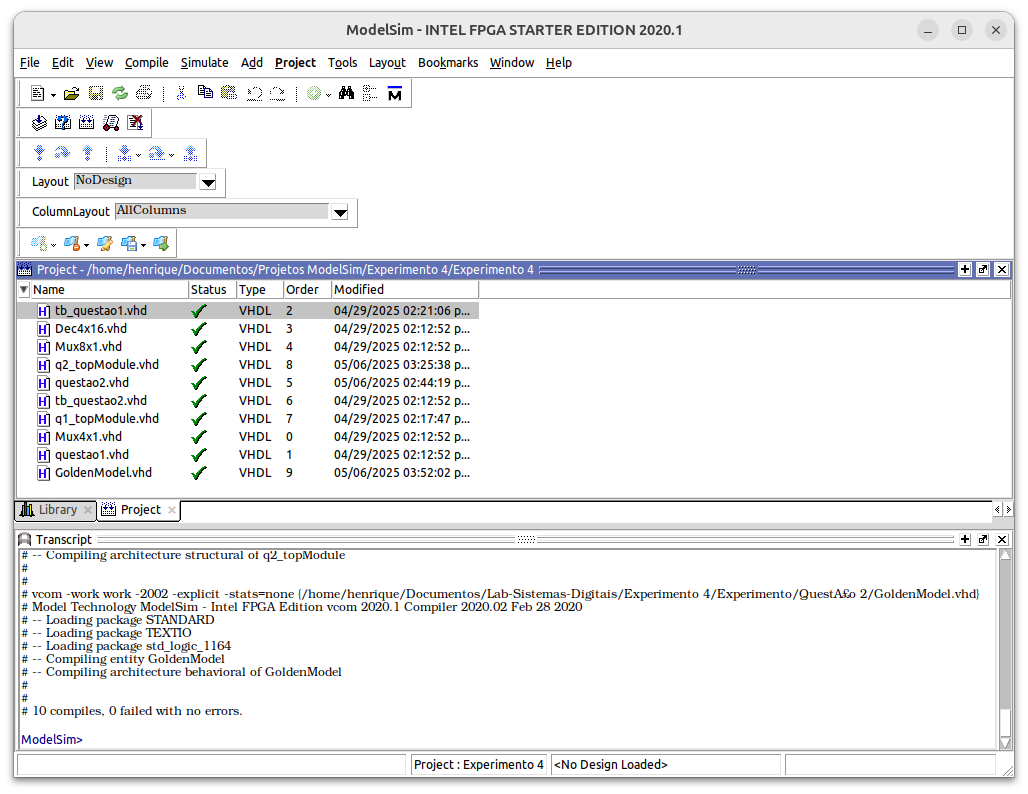
\includegraphics[width=0.75\textwidth]{Imagens/CompileModelSim.png}
    \caption{Compilação de todos os códigos apresentados}
\end{figure}

\section{Simulação}
\paragraph{}
Após compilar com sucesso os códigos apresentados, utilizamos o ModelSim para simular o comportamento dos sistemas descritos por eles. Lá, utilizamos a aba ``Waves'' para analisar o comportamento dos sinais de saída para cada combinação de valores dos sinais de entrada. A forma como as entradas variam segue o que definimos nos \textit{testbenches}, então note que as ondas referentes ao Mux 4x1 não representam todas as combinações das seis entradas. Seguem as imagens das simulações no ModelSim dos sistemas projetados.

\begin{figure}[H]
    \centering
    \begin{tcolorbox}[colframe=darkgray, colback=white, boxrule=0.5pt, arc=1pt, width=0.95\textwidth, center, boxsep=0pt, left=0pt, right=0pt]
    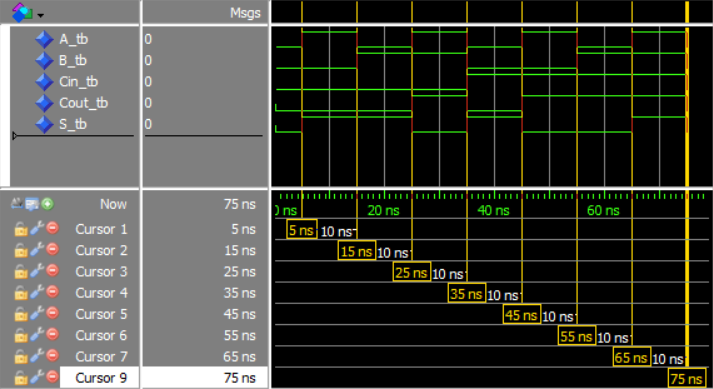
\includegraphics[width=1\textwidth]{Imagens/waves.png}
    \end{tcolorbox}
    \caption{Simulação em forma de onda binária do somador completo}
\end{figure}

\begin{figure}[H]
    \centering
    \begin{tcolorbox}[colframe=darkgray, colback=white, boxrule=0.5pt, arc=1pt, width=0.95\textwidth, center, boxsep=0pt, left=0pt, right=0pt]
    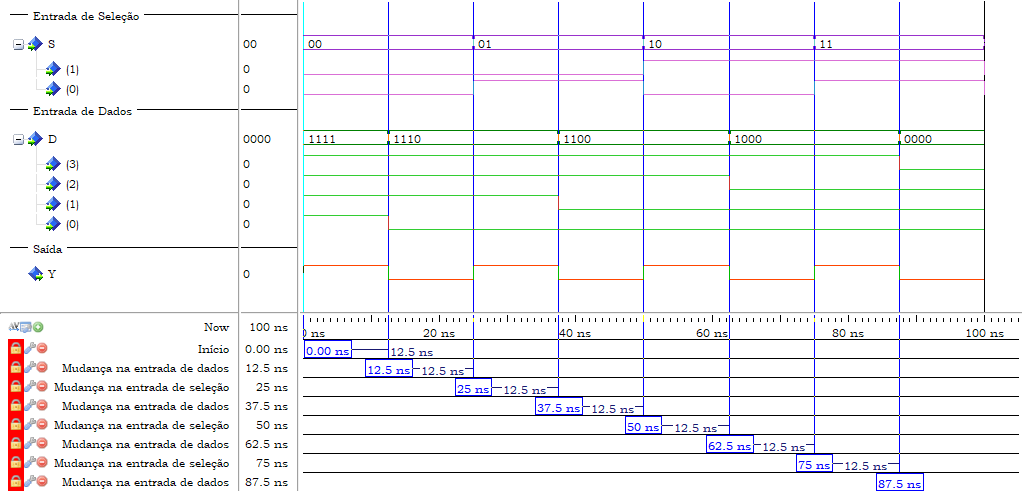
\includegraphics[width=1\textwidth]{Imagens/waves2.png}
    \end{tcolorbox}
    \caption{Simulação em forma de onda binária do multiplexador}
\end{figure}

% Análise
\section{Análise}

\paragraph{}
Para analisar os resultados obtidos, basta olhar para os valores das ondas das entradas e saídas entre cada mudança dos sinais de entrada. Os cursores estão posicionados de forma que, ao selecionar cada um deles, vemos todas as possíveis combinações das entradas e saídas correspondentes na aba à esquerda da tela.

\subsection{Análise do comportamento do Somador Completo}
\paragraph{}
 Abaixo, exibimos os \textit{prints} que denotam o comportamento dos sinais de saída $S$ e $C_{out}$ para cada combinação dos sinais de entrada $A$, $B$ e $C_{in}$.

\setlength{\fboxsep}{0pt} % Espaçamento entre a borda e a imagem
\begin{figure}[H]
    \centering
    \fcolorbox{cinza}{white}{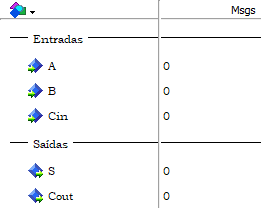
\includegraphics[width=0.3\textwidth]{Imagens/comb1.png}}
    \fcolorbox{cinza}{white}{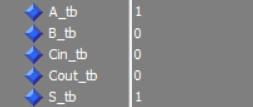
\includegraphics[width=0.3\textwidth]{Imagens/comb2.png}} \\
    \fcolorbox{cinza}{white}{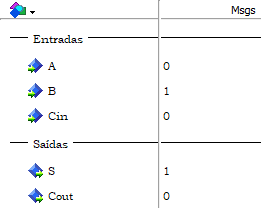
\includegraphics[width=0.3\textwidth]{Imagens/comb3.png}}
    \fcolorbox{cinza}{white}{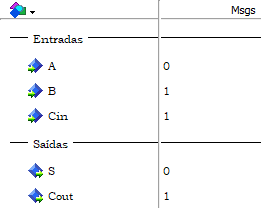
\includegraphics[width=0.3\textwidth]{Imagens/comb4.png}} \\
    \fcolorbox{cinza}{white}{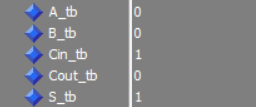
\includegraphics[width=0.3\textwidth]{Imagens/comb5.png}}
    \fcolorbox{cinza}{white}{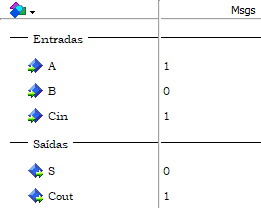
\includegraphics[width=0.3\textwidth]{Imagens/comb6.png}} \\
    \fcolorbox{cinza}{white}{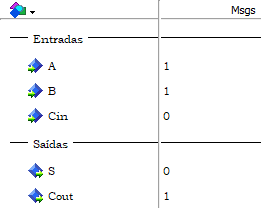
\includegraphics[width=0.3\textwidth]{Imagens/comb7.png}}
    \fcolorbox{cinza}{white}{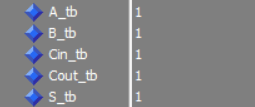
\includegraphics[width=0.3\textwidth]{Imagens/comb8.png}}
    \caption{Todas as combinações possíveis de entradas e as saídas correspondentes do Somador Completo}
\end{figure}

\paragraph{}
Percebe-se que o comportamento está de acordo com o esperado: a concatenação das saídas $C_{out}$ e $S$ corresponde à soma dos bits de entrada $A$, $B$ e $C_{in}$.

\subsection{Análise do comportamento do Multiplexador 4 para 1}

\paragraph{}
Para analisar os resultados da simulação do Mux 4x1, observou-se a saída $Y$ para cada combinação da entrada de seleção. Abaixo, estão exibidos os \textit{prints} que mostram o comportamento do circuito simulado pelo ModelSim para cada uma dessas combinações. Perceba que cada linha representa uma combinação das entradas de seleção e, portanto, uma entrada de dados selecionada, enquanto cada coluna representa um possível valor do sinal de entrada de dados selecionado.

\begin{figure}[H]
    \centering
    \includegraphics[width=0.3\textwidth]{Imagens/S=00/11.png}
    \includegraphics[width=0.3\textwidth]{Imagens/S=00/00.png} \\
    \includegraphics[width=0.3\textwidth]{Imagens/S=10/11.png}
    \includegraphics[width=0.3\textwidth]{Imagens/S=10/00.png} \\
    \includegraphics[width=0.3\textwidth]{Imagens/S=01/11.png}
    \includegraphics[width=0.3\textwidth]{Imagens/S=01/00.png}
\end{figure}
\begin{figure}[H]
    \centering
    \includegraphics[width=0.3\textwidth]{Imagens/S=11/11.png}
    \includegraphics[width=0.3\textwidth]{Imagens/S=11/00.png}
\caption{Saídas para todas as combinações das entradas de seleção e de dados selecionadas}
\end{figure}

\noindent Nota-se, em especial, os sinais destacados em cada coluna - sempre o sinal de saída $Y$ e o sinal de entrada selecionado $D_{n}$. É fácil perceber que aquele é igual a este para qualquer combinação das entradas de seleção, ou seja, que a saída é igual ao sinal selecionado, como é, por definição, em um multiplexador.

\section{Conclusão}

\paragraph{}
Nesse experimento, simulou-se, com sucesso, dois dispositivos digitais de suma importância para a eletrônica digital: o Somador Completo e o multiplexador 4 para 1. No relatório, percebeu-se o sucesso do experimento e pôde-se analisar devidamente os resultados obtidos pelas simulações, por meio das quais foi possível analisar minuciosamente esses dois circuitos e o seu comportamento para cada estímulo possível.

\paragraph{}
Concluindo, não foram observadas discrepâncias entre o comportamento esperado e o observado, podendo-se concluir, portanto, o sucesso do experimento.

\end{document}